\documentclass{standalone}
\usepackage{tikz,ctex}
\usepackage{tikz-3dplot} % 2-1
\usepackage{unicode-math} % 2-5,4-1,4-2
\setmathfont{Fira Math Regular}
\setmainfont{Fira Sans}
\definecolor{background}{RGB}{239, 239, 239} % 4-5,6-2,6-5
\begin{document}
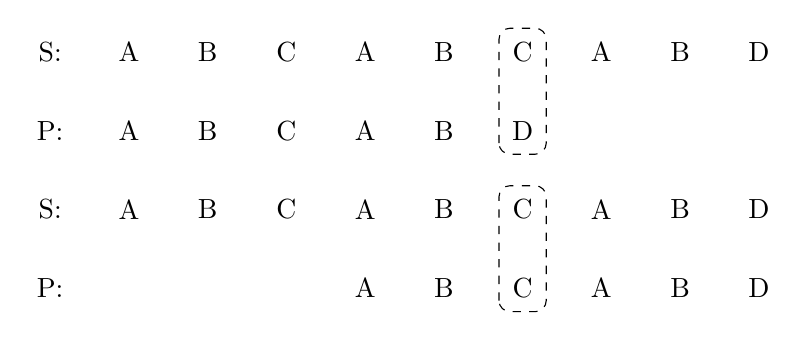
\begin{tikzpicture}
\foreach \x/\y in{1/1,1/2,1/3,4/0,4/1,4/2,4/3,7/0,7/1,7/3}{
    \node at (\x,\y) {A};
    \node at (\x+1,\y) {B};}
\foreach \x/\y in{3/1,3/2,3/3,6/0,6/1,6/3}{
    \node($2*\x+\y$) at (\x,\y) {C};}
\foreach \x/\y in{6/2,9/0,9/1,9/3}{
    \node($\x+\y-6$) at (\x,\y) {D};}
\foreach \y in {0,2}{
    \node at (0,\y+1) {S:};
    \node at (0,\y) {P:};
    \draw[dashed,rounded corners](5.7,\y-.3)rectangle(6.3,\y+1.3);}
\end{tikzpicture}
\end{document}